\chapter{Assignment: Clustering}
\label{hw:clustering}

\newthought{Clustering helps to discover groups of data}, for example similar countries based on certain socio-economic features. For this task, we will use \textit{HDI} data set from the \widget{Datasets} widget. The data reports the Human Development Index for the year 2016 for 188 countries. While HDI has its limitations, the data offers an interesting exercise in clustering.

\begin{figure}[h]
  \centering
  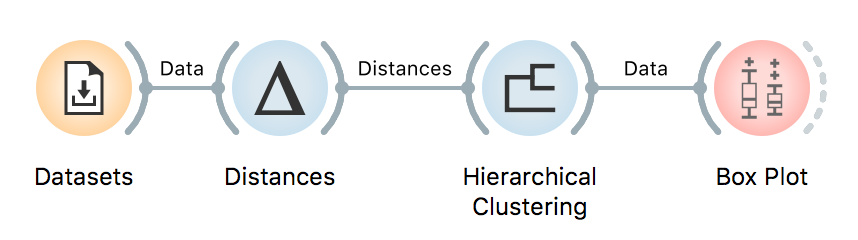
\includegraphics[width=\linewidth]{workflow.png}%
  \caption{Workflow for the assignment.}
\end{figure}

\begin{enumerate}
    \item Try Euclidean and cosine distance with Ward linkage. Which one works better? Why?
    \item How many groups did you discover? What number would make sense?
    \item Explain the final clusters. What defines each of them?
    \item Use Euclidean distance and Ward linkage. Can you explain why is Cuba clustered together with South Korea and the United Stated? Use \widget{Box Plot} and the Data output from Hierarchical Clustering to answer this question.
\end{enumerate}

\begin{wrapfigure}{o}{1.0\textwidth}
  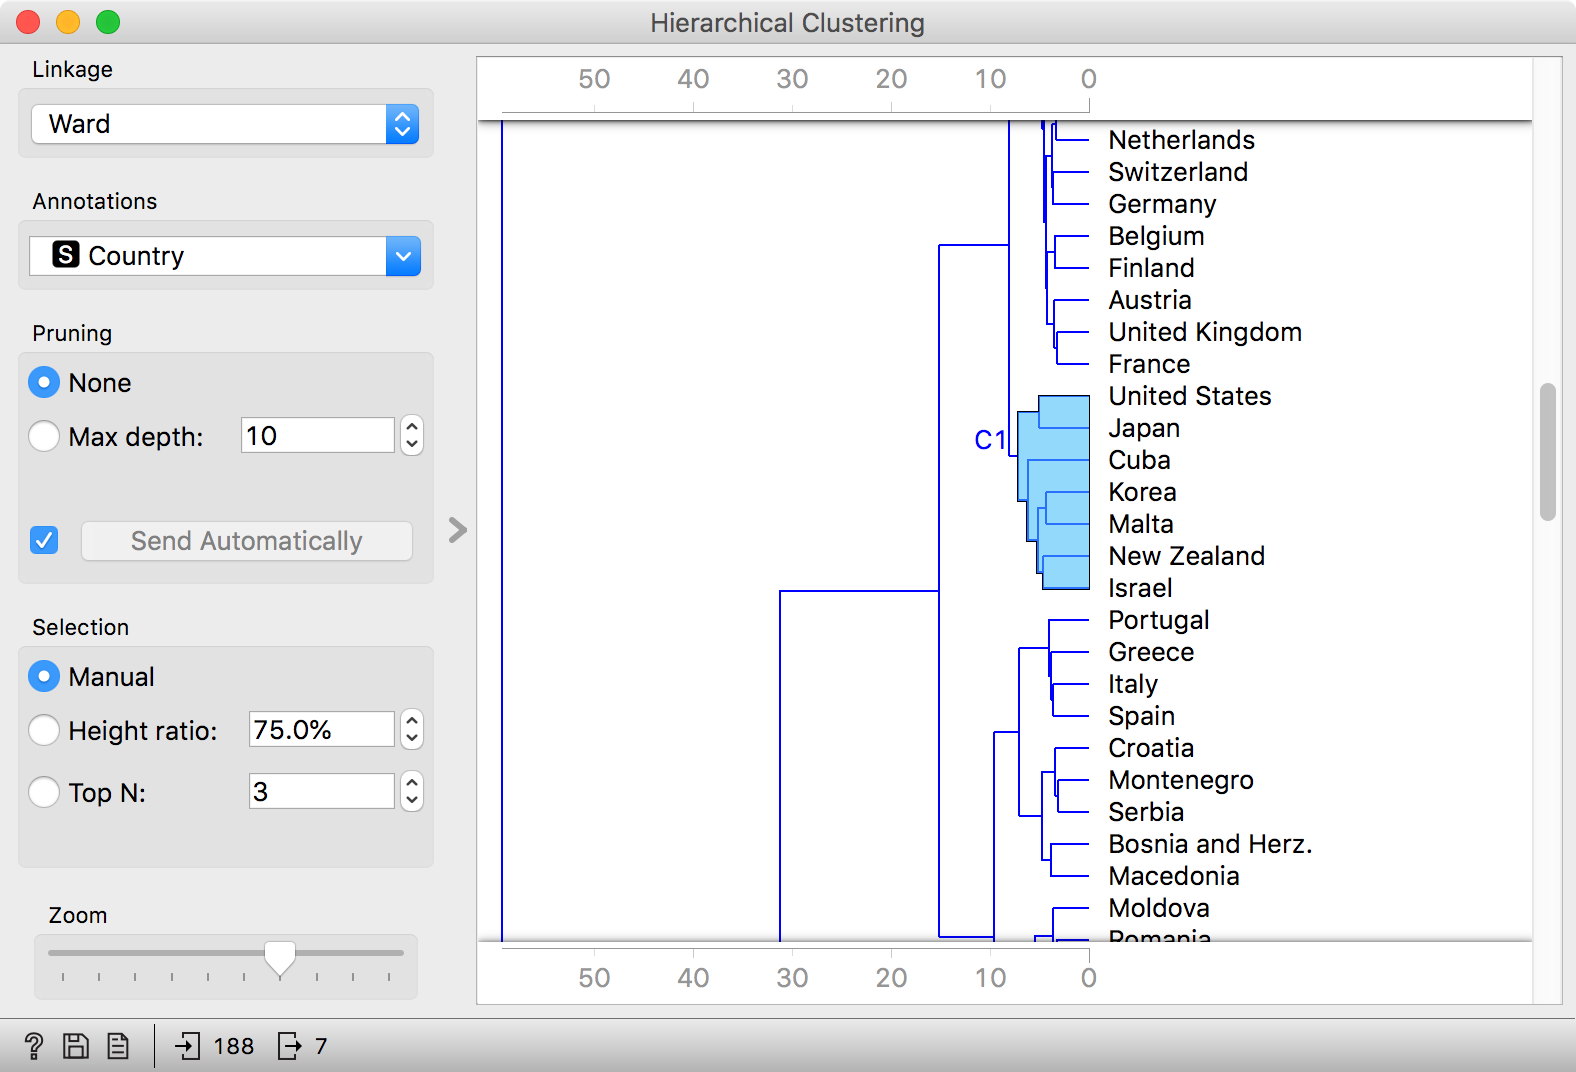
\includegraphics[scale=0.4]{clustering.png}
\end{wrapfigure}
